\documentclass[tikz,border=4pt]{standalone}
\usepackage{amsmath}
\definecolor{nod}{RGB}{31,94,165}\definecolor{clo}{RGB}{214,96,33}
\newcommand{\cuboid}[4]{% x0, height, colour, depth offset
  \fill[#3!78!black] (#1+0.32,#4,0) -- (#1+0.32,#4+0.32,0) -- (#1+0.32,#4+0.32,#2) -- (#1+0.32,#4,#2) -- cycle;
  \fill[#3!70!white] (#1,#4,0) -- (#1+0.32,#4,0) -- (#1+0.32,#4,#2) -- (#1,#4,#2) -- cycle;
  \fill[#3!25!white] (#1,#4,#2) -- (#1+0.32,#4,#2) -- (#1+0.32,#4+0.32,#2) -- (#1,#4+0.32,#2) -- cycle;
  \draw[#3!50!black,line width=0.4pt,line join=round] (#1,#4,0) -- (#1+0.32,#4,0) -- (#1+0.32,#4+0.32,0) -- (#1+0.32,#4+0.32,#2) -- (#1,#4+0.32,#2) -- (#1,#4,#2) -- cycle (#1,#4,#2) -- (#1+0.32,#4,#2) -- (#1+0.32,#4+0.32,#2) (#1+0.32,#4,#2) -- (#1+0.32,#4,0);
}
\begin{document}
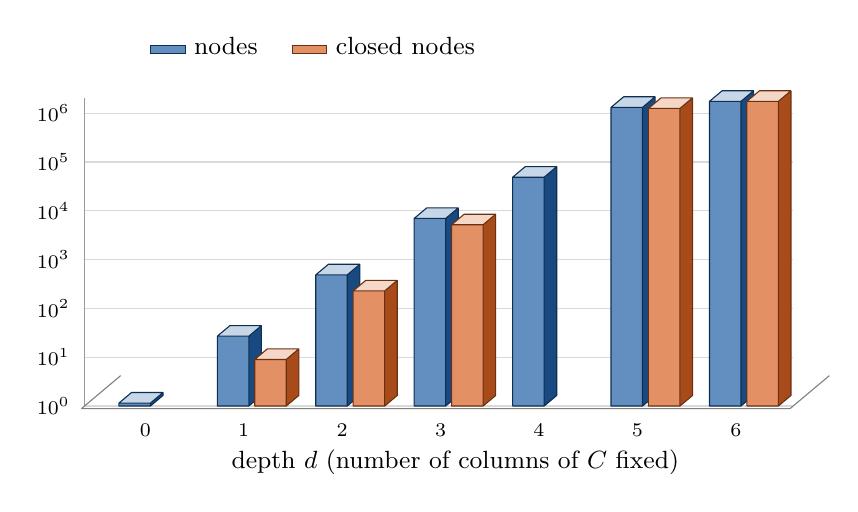
\begin{tikzpicture}[x={(1.25cm,0cm)},y={(0.5cm,0.42cm)},z={(0cm,0.62cm)},font=\small]
\foreach \k in {0,...,6} { \draw[black!15] (-0.2,0.08,\k) -- (7.0,0.08,\k); \node[anchor=east,font=\scriptsize] at (-0.25,0.08,\k) {$10^{\k}$}; }
\draw[black!40] (-0.2,0.08,0) -- (-0.2,0.08,6.3);
\draw[black!50] (-0.2,0,0) -- (7.0,0,0) -- (7.0,1,0) (-0.2,0,0) -- (-0.2,1,0);
\cuboid{0.15}{0.060}{nod}{0.08}
\node[font=\scriptsize] at (0.45,0,-0.45) {0};
\cuboid{1.15}{1.431}{nod}{0.08}
\cuboid{1.53}{0.954}{clo}{0.08}
\node[font=\scriptsize] at (1.45,0,-0.45) {1};
\cuboid{2.15}{2.687}{nod}{0.08}
\cuboid{2.53}{2.358}{clo}{0.08}
\node[font=\scriptsize] at (2.45,0,-0.45) {2};
\cuboid{3.15}{3.843}{nod}{0.08}
\cuboid{3.53}{3.713}{clo}{0.08}
\node[font=\scriptsize] at (3.45,0,-0.45) {3};
\cuboid{4.15}{4.687}{nod}{0.08}
\node[font=\scriptsize] at (4.45,0,-0.45) {4};
\cuboid{5.15}{6.118}{nod}{0.08}
\cuboid{5.53}{6.096}{clo}{0.08}
\node[font=\scriptsize] at (5.45,0,-0.45) {5};
\cuboid{6.15}{6.241}{nod}{0.08}
\cuboid{6.53}{6.241}{clo}{0.08}
\node[font=\scriptsize] at (6.45,0,-0.45) {6};
\node at (3.6,0,-1.1) {depth $d$ (number of columns of $C$ fixed)};
\node[anchor=west] at (0.2,0.5,7.1) {\tikz\fill[nod!70!white,draw=nod!50!black] (0,0) rectangle (0.25,0.25); nodes \quad \tikz\fill[clo!70!white,draw=clo!50!black] (0,0) rectangle (0.25,0.25); closed nodes};
\end{tikzpicture}
\end{document}
